\documentclass[11pt,letterpaper]{article}
%\usepackage{amsmath}
\usepackage{graphics}
\usepackage{fullpage}
\addtolength{\voffset}{0.5in}

%
%  Cool LaTeX resource:
%   http://en.wikibooks.org/wiki/LaTeX

\begin{document}
\title{Models of student learning and multimodel inference}
\author{Brett van de Sande}

\maketitle

\begin{abstract}
We compare several models of student learning with the goal of 
determining when a specific student has learned a particular skill.  
We use Likelihood Theory to determine
which of several models best describes the acquisition
of skills associated with introductory physics.  Then we
use a multimodel approach to determine the relative probability
that a student has learned a given skill at a particular 
problem-solving step.  Finally, we relate this
approach with Hidden Markov model based approaches like
Bayesian Knowledge tracing.
\end{abstract}

\section{Introduction}

Talk about ultimate goal of using this to determine effectiveness
of help given or of a particular student behavior.

Survey of BKT work done to date.

\section{A model of learning}

Define steps and transactions.

For each student and KC, the student has attempted some number of 
{\em steps} that involve that KC.   We will label
steps with $j$.  Usually a given step is associated
with a single user interface object (an equation, vector, etc.)  but
not always, since a student may attempt a particular problem solving
step, delete the object, and later attempt that solution step again.
Each step $j$ corresponds some some number of student-tutor 
{\em transactions}: attempts at constructing the associated object, 
or associated interactions with the Andes help system.  

%Next, we need a model of student learning for a particular KC.
%Since the policies chosen by the random-help version of Andes
%are different for each student,
%we need to determine the point of learning for each student.
For each KC and student, mark each step as ``correct'' if
the student completes the step correctly without any associated errors or 
requests for help; otherwise, the step is marked as ``incorrect.''
\label{steps} 
%
% From Kurt:
Thus, if each incorrect/correct step is marked with a 0/1, then
a single student's performance on a single KC is a bit string,
{\em exempli gratia} 00101011.

\section{Three models of learning}

In order to determine when a student has learned a particular still,
we need to introduce a model of learning for that student and skill.
Ideally, the model should have the the following properties:
\label{model-criteria}
%
\begin{enumerate} 

\item Be compatible with actual student behavior.
      See Section~\ref{model-selection}.

\item \label{crit:step}
      Give the probability that learning has occurred at a given step.
      See Section~\ref{multi-model}.

\item  \label{crit:perform}
      Assuming learning has occurred at a given step, give the 
     associated increase in performance and 
     the rate of errors after learning.

\end{enumerate}
%
We will consider three candidate models:  the ``step model,'' 
the logistic function, and the Bayesian Knowledge Tracing model.

The ``step model'' assumes that learning occurs all at 
once~\cite{aha-moments}.  It is defined as:
%
\begin{equation}
    P_\mathrm{step}(j)= \left\{\begin{array}{cc}
                 g, & j<l \\
                 1-s, & j\ge L 
                 \end{array} \right. 
\end{equation}
%
where $L$ is the step where the student first shows mastery of the
KC, $g$ is the ``guess rate,'' the probability that the student
gets a step correct by accident, and $s$ is the ``slip rate,''
the chance that the student makes an error after learning
the skill.  These are analogous to the guess and slip parameters 
of Bayesian Knowledge Tracing~\cite{anderson}.  
The associated gain in performance
is $1-g-s$ and the error rate after learning is simply $s$ in this
model.  Thus, this model satisfies criteria \ref{crit:step} and
\ref{crit:perform}.

Another model that is frequently used in the context of 
learning is the logistic model~\cite{logit},
%
\begin{equation}
    P_\mathrm{logit}(j)= \frac{1}{1+\exp\left(-b (j-L)\right)} \; .
\end{equation}
%
It is natural to associate $L$ with the moment of learning.  However,
the finite slope $P_\mathrm{logit}(j)$ means that learning may occur
in a range of roughly $1/b$ steps before and after $L$.    For  
$P_\mathrm{logit}(j)$, the gain in performance is always 1 and the final error
rate is always 0.  Thus although this model makes a prediction for
when the skill is learned, criterion~\ref{crit:step}, it does
not predict a gain in performance, criterion~\ref{crit:perform}.

The third model is the Bayesian Knowledge Tracing (BKT) model~\cite{anderson}.
Although this model is usually expressed as a Hidden Markov model, 
one can express it in terms of its solution (see Appendix~\ref{bkt}),
which is an exponential,
%
%  A and \beta are kind of messy, so we don't include them here.
\begin{equation}
         P_\mathrm{BKT}(j) = 1-P(S) -A e^{-\beta j} \; .
\end{equation}
%
One central assumption of BKT is that, given that learning
has not already occurred, mastery is {\em equally probable} on each step.
This assumption of equal probability does not match well with 
our goal of determining empirically the steps where learning has 
actually occurred, criterion~\ref{crit:step}.
On the other hand, this model does provide initial and final
error rates, so criterion~\ref{crit:perform} is satisfied. 

\section{Model selection using AIC}
\label{model-selection}

Although this will not determine our choice of model in subsequent
work, it would be reassuring to know whether the step model 
$P_\mathrm{step}(j)$
describes the student data as well (or better than) the
other two models, $P_\mathrm{logit}(j)$ and $P_\mathrm{BKT}(j)$.  
We believe that the Akaike Information 
Criterion (AIC) is the most appropriate metric~\cite{akaike,aicbook}
to use for this purpose.

\subsection{Method}


\begin{figure}
  \centering 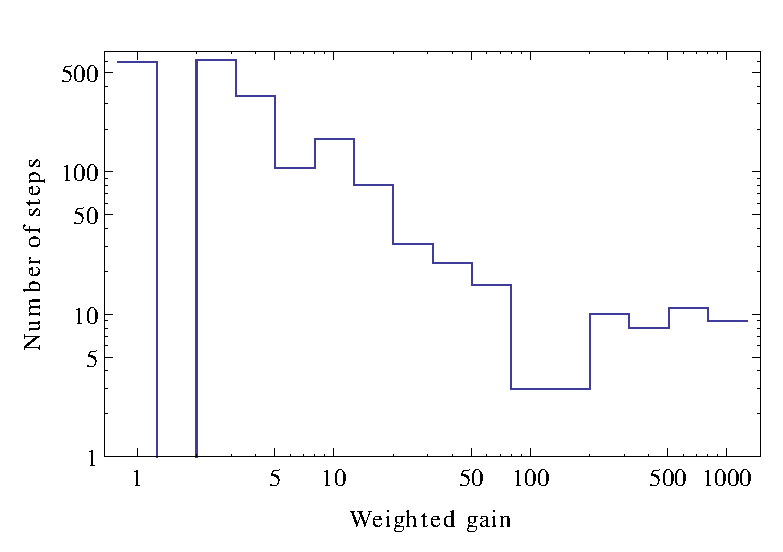
\includegraphics{student-kc-length-histogram.eps}
  \caption{Histogram of number of student-KC pairs in the student 
    dataset having a given number of steps.}
    \label{student-length-histogram}
\end{figure}

We examined log data from 12 students taking an intensive 
introductory physics course at St.\ Anselm College during
summer 2011.  The course
covered the same content as a normal two-semester introductory
course.  Log data was recorded as students solved homework 
problems while using the Andes intelligent tutor homework system.
231 hours of log data were recorded.
%, covering 85,744 transactions, and 26,204 student steps.  
Each step was assigned to one or more different KC's.  
The dataset contains a total of 2017 distinct
student-KC pairs covering a total of 245 distinct KC's.
See Figure~\ref{student-length-histogram} for a histogram
of the number of steps.

Most KC's are associated with physics
or relevant math skills while others are associated with 
Andes conventions or user-interface actions (such as, notation
for defining a variable).  The student-KC pairs with the largest 
number of steps are associated with user-interface related skills,
since these skills are exercised throughout the entire course. 

The presence of many student-KC pairs with just one or two
steps suggests that the cognitive model associated with this tutor
system may be sub-optimal; there has not been any attempt, to date,
to improve on the cognitive model of Andes with, say, Learning 
Factors Analysis~\cite{lfa}.

\subsection{Analysis}

Since the goodness of fit criterion, AIC, is valid in the limit 
of many steps, we include in this analysis only student-KC 
pairs that contain 10 or more turns, reducing the number of 
student-KC pairs to 267, covering 38 distinct KC's.
We determine the correctness of each step (Section~\ref{steps}),
assigning a 1 if the step is correct or 0 if it is not.
Thus, for each student-KC pair, we construct bit string, {\em exempli gratia},
001001101.  This bit string is then fit to each of the three models,
$P_\mathrm{step}(j)$, $P_\mathrm{logit}(j)$, and $P_\mathrm{BKT}(j)$ by
maximizing the associated log likelihood.  
%This determines the free parameters in each model. 
We then calculate the corrected AIC score, AIC$_\mathrm{c}$~\cite{aicbook} 
for each fit.  
Finally, we calculated the Akaike weights, $w_\mathrm{logit}$,
$w_\mathrm{step}$, and $w_\mathrm{BKT}$ for each student-KC pair.  
The Akaike weight represents the relative probability that
a particular model in a given set of models most closely matches
the true model that has actually generated the data.
The weights are normalized so that 
%
\begin{equation}
   1=w_\mathrm{logit}+ w_\mathrm{step} + w_\mathrm{BKT} \; .
\end{equation}
%
A scatter plot of the weights is shown in Fig.~\ref{scatter1}.
Since a student-KC pair contains only an average of about 16 steps, we 
expect that AIC$_\mathrm{c}$ should not strongly
discriminate between the models.  Instead, we expect that
any statistically significant difference will only appear 
after including hundreds of student-KC in our sample.  However, 
this is not what we found; instead, we see that $P_\mathrm{BKT}$ is 
strongly disfavored over $P_\mathrm{step}(j)$ and $P_\mathrm{logit}(j)$.
Perhaps this result is too good to be true?

\begin{figure}
  \centering 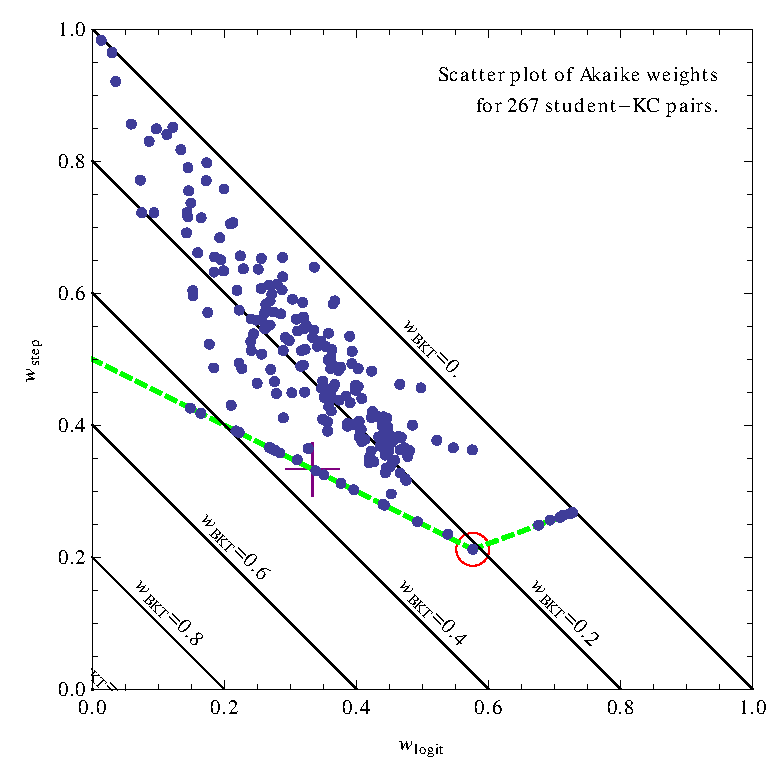
\includegraphics{scatter-weights.eps}
  \caption{Scatter plot of  Akaike weights for the three models, 
   $P_\mathrm{step}$, $P_\mathrm{logit}$, and $P_\mathrm{BKT}$, 
   when fit to 267 student-KC pairs from an introductory physics course.
   The model $P_\mathrm{BKT}$ seems to be highly disfavored over
   the other two models; however, we believe this result
   may be spurious.} \label{scatter1}
\end{figure}

To further investigate this situation, we constructed an
artificial dataset containing 100 random bit strings (each
step has 50\% probability of being ``correct'') of 100 steps each.
This dataset corresponds to a model of the form
%
\begin{equation}
        P_\mathrm{random}(j)=1/2 \; .
\end{equation}
%
We then repeated our analysis of the three models using this
dataset.  In this case, one expects that all three models 
should perform equally well since all three can equal 
(with suitable choice of parameters) the known correct model 
$P_\mathrm{random}(j)$.
Thus, we would expect a scatter plot of the Akaike weights to 
center around 
$w_\mathrm{logit}=w_\mathrm{step}=w_\mathrm{BKT}=1/3$.
Instead, we find that $P_\mathrm{step}$ is highly favored over
the other two; see Fig.~\ref{scatter2}.  
This indicates that there are large non-leading
corrections to the AIC$_\mathrm{c}$ that have not been
taken into account.  Burnham \& Johnson conclude 
that there is more work to be done in this area~\cite[p.~380]{aicbook}: 
``Operating characteristics
of AIC-based model selection for count-type data need more 
more study for small sample sizes.''  Apparently, 100 data points
is still too small.

\begin{figure}
  \centering 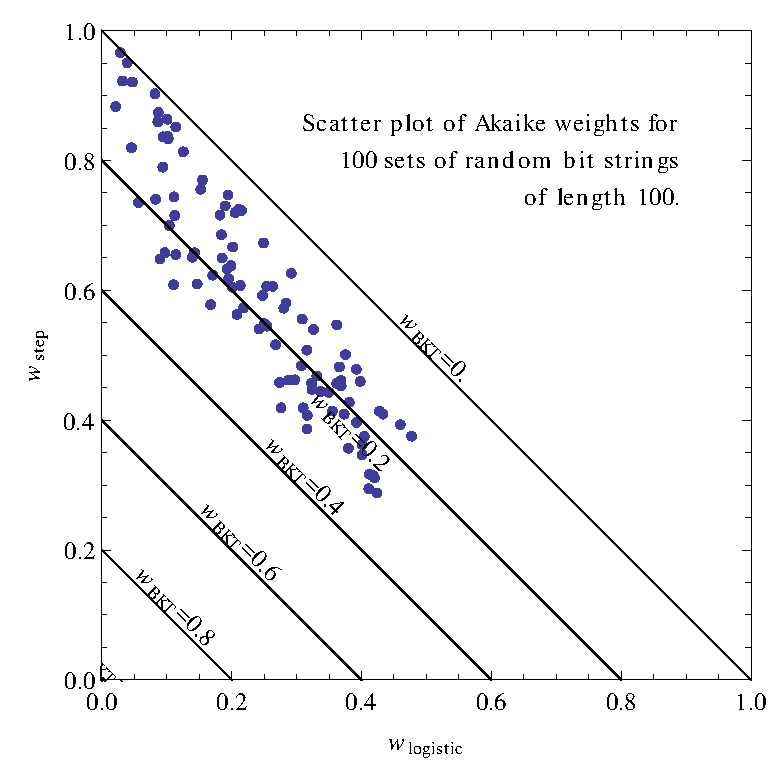
\includegraphics{scatter-random-weights.eps}
  \caption{Scatter plot of Akaike weights for the three models, 
   $P_\mathrm{step}$, $P_\mathrm{logit}$, and $P_\mathrm{BKT}$, 
   when fit to randomly generated data.  For this dataset, each 
   model should perform
   equally well; the large bias in favor of one model indicates
   that  AIC$_\mathrm{c}$ is failing.}\label{scatter2}
\end{figure}

\subsection{Summary}

In conclusion, the most powerful technique for model selection,
AIC, fails to to properly distinguish models when the random
variable (the dataset) is binary-valued (Bernoulli trials),
the sample sizes are small (10 to 100 points), and the models
have very different functional forms.  Since the use of such
models is foundational to KC-based approaches to Educational
Data mining, we believe that it is imperative that this issue 
associated with model selection must be resolved.

Demonstrating that the step model fits student data as well as,
or better than, the other two would be an
{\em ex post facto} justification for using that model.  
However, our use of the step model is primarily motivated
by criteria~\ref{crit:step} and \ref{crit:perform} of 
Section~\ref{model-criteria}.
In Section~\ref{multi-model}, we show how AIC-based methods
can yield the probability that learning has occurred during given step.

\section{Multi-model approach}
\label{multi-model}

We need to determine the step where a specific student has learned a
particular skill.  Our strategy is to take the step model, 
$P_\mathrm{step}(j)$, and treat $L$ as a constant, yielding a set of 
sub-models $P_{\mathrm{step},L}(j)$.
We then fit each of the sub-models to the student data, obtaining an
AIC value.  Finally, we find the Akaike weighs for each of the
sub-models.  The Akaike weights gives that probability that learning
occurred at each step.

\begin{figure}
  \centering 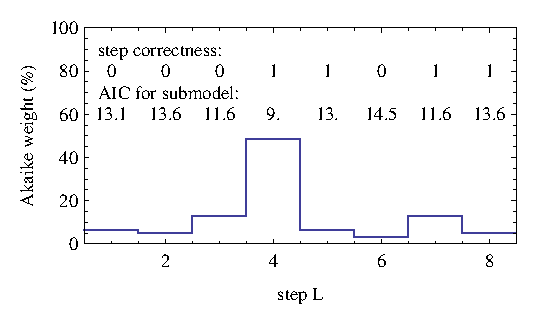
\includegraphics{step-weights.eps}
   \caption{Akaike weights for the submodel $P_\mathrm{step}(j)$
      where $L$ is fixed.  This gives the relative probability that
      the student learned the KC just before step $L$.}
    \label{step-weights}
\end{figure}

Let us illustrate this technique with a simple example. 
Suppose the bit-string for a particular student-KC pair is 
00011011 (8 opportunities); see Fig.~\ref{step-weights}.
We fit this datum to 8 sub-models of the step model, corresponding to
$L\in\{1,2,\ldots,8\}$, by maximizing the likelihood $\mathcal{L}$.  
The associated AIC values are
given by $\mathrm{AIC}_L=2 K-\log \mathcal{L}$  where $K$ is the
number of fit parameters.  When $L>1$, $K=2$  (parameters $s$ and $g$) and 
when $L=1$, $K=1$ (paramter $s$ only).
%
%\begin{table}
%\caption{
%\begin{tabular}{crrrrrrrr}
% opportunity & 1 & 2 & 3 &4 & 5 & 6 & 7 & 8 \\
 % AIC &   13.1 & 13.6 & 11.6 & 9.0 & 13.0 & 14.5 & 11.6 & 13.6 \\
%\end{tabular}
%\end{equation}
%
Not suprisingly, the best fit (lowest AIC) corresponds to the first
1 in the dataset at step~4.  From the AICs, we calculate the Akaike weights
%
\begin{equation}
     w_L=\frac{e^{-\mathrm{AIC}_L/2} }{\sum_{L^\prime}
       e^{-\mathrm{AIC}_{L^\prime}/2}} \; .
\end{equation}
%

Note that the case $L=1$ corresponds to the student having 
``learned the skill'' some time before the first step.  That is to say, 
the student does not acquire the skill while using the tutor system.
Thus, $w_{L=1}$ should be interpreted as the relative probability
that no learning has occurred while using the tutor system.

\section{Model Effectiveness}

Our ultimate goal is to distinguish steps that result in 
learning from steps that do not.  Hopefully, one can use this
information to infer something about the effectiveness of the help
given on a particular step, or the effectiveness of
the student activity on that step.

\begin{figure}
  \centering 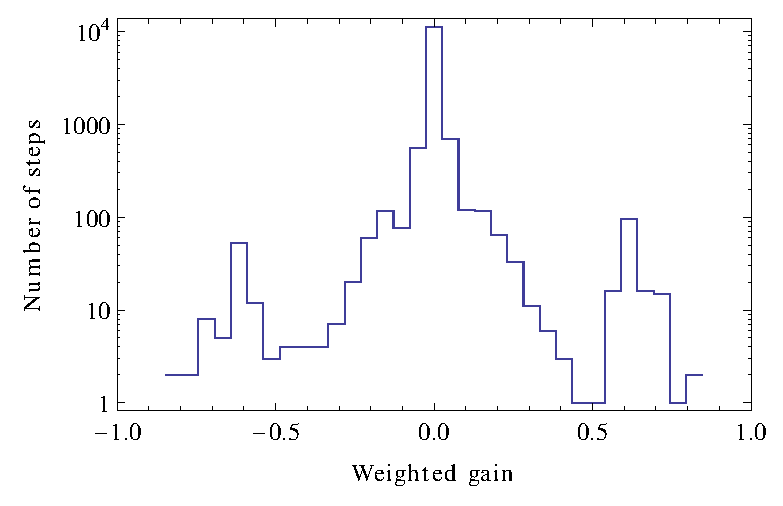
\includegraphics{weighted-gain-histogram.eps}
   \caption{Histogram of weighted gains $w_L \Delta_L$ for
     all steps in all student-KC pairs in the student dataset.}
    \label{weighted-gain-histogram}
\end{figure}

In using the weights to determine whether a specific step $L$
is ``good'' or ``bad'' for learning, we will use the Akaike
weight times the associated learning gain, $w_L \Delta_L$.
The learning gain $\Delta_L=1-\hat{g}-\hat{s}$ where $\hat{g}$ and $\hat{s}$
are the Maximum Likelihood estimators for $g$ and $s$ given
by submodel  $P_{\mathrm{step},L}(j)$.  We define the ``no learning''
case, $\Delta_1=0$.
We will call  $w_L \Delta_L$ the ``weighted gain'' associated with 
$P_{\mathrm{step},L}(j)$.
A histogram of $w_L \Delta_L$ for the student dataset is
shown in Fig.~\ref{weighted-gain-histogram}.

We propose to use the average of the weighed gains as
a ``quality index'' $Q$ for determining how suitable a 
dataset is for determining the point of learning for an individual
student-KC pair:
%
\begin{equation}
           Q= \frac{1}{N} \sum_\alpha \sum_L w_L \Delta_L
\end{equation}
%
where $\alpha$ is an index running over all student-KC pairs in a 
dataset and $N$ is the number of student-KC pairs.
For random data, we expect the distribution of weighted gains
to be symmetric about zero and $Q$ to be zero. 
For the best possible data (with the form $00\cdots011\cdots1$), 
we expect the maximum value of $w_L$ to be nearly 1 
with associated $\Delta_L\approx 1$ so that $Q\approx 1$.

Returning to our student dataset, we find $Q=0.074\pm0.014$, which
is small, but significant.  Let us compare this to an artificially
constructed ideal dataset (as describe above) with a similar number 
of steps as the student dataset, we get $Q=0.81\pm0.01$.  For 
a datset where we take the student dataset and randomly
reorder the steps, we get $Q=-0.004\pm0.004$, consistent with zero.

\section{Conclusion}

One thing that we can conclude is that determining the
moment of learning for an individual student is a murky
business, as can be seen by comparing the weighted gains for
the student dataset to the weighted gains of a 
randomly generated dataset.

However, the fact that we can find significant positive average gains,
suggests the situation is not hopeless.  We can use $Q$ to determine
the predictive power of a given dataset. 

%%%%%%%%%%%%%%%%%%%%%%%%%%%%%%%%%%%%%%%%%%%%%%%%%%%%%%%%%%%%%%%%%%
\appendix
\section{Bayesian Knowledge tracing}
\label{bkt}

The Bayesian Knowledge tracing model~\cite{anderson} has four parameters:
%
\begin{itemize}
   \item $P_0$ is the initial probability of knowing a skill.
   \item $P(G)$ is probability of guessing correctly, if the student        
         doesn't know the skill.
   \item $P(S)$ is probability of slips, if student does know the skill.
   \item $P(L)$ is probability of learning the skill if the student 
         does not know the skill.  Note that this is assumed to 
         be constant over steps.
\end{itemize}
%
Let $P_j$ be the probability that the student knows the skill at 
step $j$. According to the model,  $P_j$ can
be determined in terms of the previous opportunity:
%
\begin{equation}
          P_j = P_{j-1} + P(L)\left(1-P_{j-1}\right)
\end{equation}
%
According to this model, the probability that the student actually gets
opportunity $j$ correct is:
%
\begin{equation}
        P_\mathrm{BKT}(j) = P(G)\left(1-P_j\right) + 
                     \left(1-P(S)\right) P_j \label{pnc}
\end{equation}
%
(Unlike the four model parameters above, there isn't a consistent
notation for $P_\mathrm{BKT}(j)$ in the literature.)
This model can be exactly solved with solution: 
%
\begin{equation}
            P_j = 1-\left(1-P(L)\right)^j\left(1-P_0\right)
	    \label{sol}
\end{equation}
%
%
Substituting (\ref{sol}) into (\ref{pnc}), we get:
%
\begin{equation}
         P_\mathrm{BKT}(j) = 1-P(S) -\left(1-P(S)-P(G)\right) \left(1-P_0\right)
                   \left(1-P(L)\right)^j \label{pncsoln}
\end{equation}
%
Note that the functional form of $P_\mathrm{BKT}(j)$ is a function of {\em three}
parameters:  $P(S)$, $P(L)$, and $\left(1-P(S)-P(G)\right) \left(1-P_0\right)$.
This degeneracy of the model was first noticed by Beck and 
Chang~\cite{beckchang}.  In their paper, they notice that multiple
combinations of $P(G)$ and $P_0$ give exactly the same $P_\mathrm{BKT}(j)$, but
fail to explain why this is the case.

\begin{figure}
  \centering 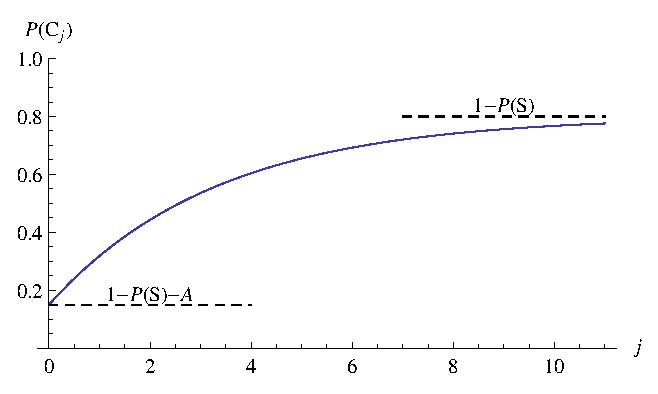
\includegraphics{exponential.eps}
   \caption{The graph of the solution of the Bayesian Knowledge
     Tracing model.}
    \label{bkt-function}
\end{figure}

The functional form of (\ref{pncsoln}) is an exponential.
If we define 
$A=\left(1-P(S)-P(G)\right) \left(1-P_0\right)$ and
$\beta=-\log(1-P(L))$, then we can rewrite (\ref{pncsoln}) in 
a clearer form:
%
\begin{equation}
         P_\mathrm{BKT}(j) = 1-P(S) -A e^{-\beta j}
\end{equation}
%
In conclusion, Bayesian Knowledge tracing is equivalent to using
an exponential function with three parameters to fit the student data;
see Fig.~\ref{bkt-function}


%Equations (1) and (2) of \cite{brunskill} 
%are equivalent to the first three equations in \cite{baker}
%\begin{eqnarray}
%   P(L_n|\mbox{correct}) &=& P(T)+\frac{\left(1-P(T)\right) P(L_{n-1})
%          \left(1-P(S)\right)}
%               {P(L_{n-1})\left(1-P(S)\right)+\left(1- P(L_{n-1})\right) P(G)}\\
%   P(L_n|\mbox{incorrect}) &=& P(T)+\frac{\left(1-P(T)\right) P(L_{n-1})
%          \P(S)\right}
%               {P(L_{n-1})P(S)+\left(1- P(L_{n-1})\right) \left(1-P(G)\right)}\\
%with the substitution:
%
%\begin{equation}
%         P(L_{n-1}) \to P(T)+\left(1-P(t)\right) p(L_t)
%\end{equation}
%
%This equivalence is from changing the order of updating
%student mastery and updating the estimate based on student
%response, as noted by the authors.  However, this raises
%a question for Equations (3) and (4) of \cite{brunskill}.
%Should the probability be taken before or after updating the
%student mastery:



\begin{thebibliography}{9}

\bibitem{anderson} 
  Corbett, A.\ T., Anderson, J.\ R. Knowledge Tracing:  Modeling 
the Acquisition of Procedural Knowledge.  \emph{User Modeling and
 User-Adapted Interaction}, 1995, 4, 253--278.

\bibitem{beckchang}
  Beck, J.\ E., Chang, K.-m.\ Identifiability: A Fundamental Problem of
  Student Modeling.
  \emph{Proceedings of the $11^{th}$ International Conference on User 
    Modeling}, 2007.

\bibitem{baker} Baker, R, Corbett, A., Aleven, V.,  Improving Contextual 
    Models of Guessing and Slipping with a Truncated Training Set. 
    First International Conference on Educational Data Mining. 2008. 

\bibitem{brunskill}
   Lee, J.\ I., Brunskill, E.\ The impact of Individualizing Student 
  Models on Necessary Practice Opportunities.  EDM, 2012.

\bibitem{logit}
  Ken Koedinger paper, other papers, using logistical regression.
  Min Co-author on some?

\bibitem{akaike}
   Akaike original paper

\bibitem{aicbook}
   Burnham \& Johnson book

\bibitem{aha-moments}
   Baker, R.S.J.d., Goldstein, A.B., Heffernan, N.T. (2011) 
     Detecting Learning Moment-by-Moment. International Journal of 
    Artificial Intelligence in Education, 21 (1-2), 5-25.
   % http://users.wpi.edu/~rsbaker/BGH-IJAIED-v29.pdf

\bibitem{lfa}
  H. Cen, K. Koedinger and B. Junker, Learning Factors Analysis - A General Method for Cognitive Model Evaluation and Improvement, 8th International Conference on Intelligent Tutoring Systems, 2006. 
  % www.ml.cmu.edu/research/dap-papers/cen_kddpaper2.pdf

\end{thebibliography}




\end{document}